\documentclass{article} % Try also "scrartcl" or "paper"
\usepackage{blindtext} % for dummy text
\usepackage{polski}
\usepackage[utf8]{inputenc}
\usepackage{listings}

\usepackage{graphicx}
% \usepackage[margin=2cm]{geometry}   % to change margins
% \usepackage{titling}             % Uncomment both to   
% \setlength{\droptitle}{-2cm}     % change title position 
\author{Piotr Piękos}
\title{%\vspace{-1.5cm}            % Another way to do
Premise selection with machine learning}
\begin{document}
\maketitle

\section{Introduction}

Task description is in a file Task.pdf

 The goal was to create a premise selection machine learning algorithm from the mizar dataset based only on obfuscated binary features. 
 
 Several models are created with similar pipeline and next steps are suggested.
\section{General Description}
	
Approach is as follows:
\begin{enumerate}
\item Features are translated into numeric table (with memory-efficient types to make it possible)
\item Dataset of lists of theorems and premises is split into pairs of theorems and premises, so we ignore "set dependencies" - we don't predict usefulness for sets, just for single premises.
\item features from premise and theorem are concatenated
\item model on that dataset is trained to predict usefulness of the feature.
\end{enumerate}

Whole processing is in \textit{'notebooks/training.ipynb'} 
(some parts were done with LGBM CLI after saving datasets to LIBSVM format, because lgbm python interface takes much more RAM).

Results are analysed in \textit{'notebooks/compare\_results.ipynb'}

\section{Dataset creation}

As mentioned above, lists of premises for theorems are translated into pairs (theorem, pair). Rows created with that manner are labeled with 1 for usefulness. 

Additional N rows (N is a hyperparameter) are sampled per every theorem from premises that aren't in "useful" set.

\subsection{Embeddings} 

Additionally dense features are created with autoencoders. They are not used in every model though.

Before training simple autoencoder with two layers (ReLU, sigmoid) on the theorem/feature matrix - the reasoning is that similar features give similar 'context' for premises.

One could also try to do embeddings based theorem-premise relationships

\section{Models}


6 LGBM models and 1 RF models are tested.
5 LGBM models and RF model are on raw data, 1 LGBM model is on AutoEncoder Embeddings.
One of the LGBM models is on embeddings from AutoEncoder

LGBM differ in hyperparameters, hyperparameters sets:
(shallow, deep, naive)  \newline\
\textbf{NAIVE Hyperparameters}
\begin{lstlisting}[language={}]
output_model=LGBM_params_naive.bst
objective = binary
metric = auc
is_unbalance = true
boosting = gbdt
max_depth = 80
learning_rate = 0.05
num_rounds = 300
data = train.libsvm

\end{lstlisting}


\textbf{SHALLOW Hyperparameters}
\begin{lstlisting}[language={}]
output_model=LGBM_params_shallow.bst
objective = binary
metric = auc
is_unbalance = true
boosting = gbdt
num_leaves = 30
feature_fraction = 0.75
bagging_fraction = 0.8
bagging_freq = 20
learning_rate = 0.035
lambda_l2 = 0.06
verbose = 1
nthreads = 6
max_bin = 255
num_rounds = 5000
data = train.libsvm
\end{lstlisting}
\textbf{DEEP Hyperparameters are basically the same but without restriction on num leaves}


Following models are tested:
(If not stated otherwise there are 8 false clauses per every positive clause)
\begin{itemize}
\item lgbmnaive- lightgbm trained with NAIVE hyperparameters
\item lgbmshallow - lightgbm trained with SHALLOW hyperparameters
\item lgbmdeep - lightgbm trained with DEEP hyperparameters
\item lgbmdeepshallowmean - average of predictions of lgbmdeep and lgbmshallow
\item lgbmdeepshallowmean\_16 - average of predictions of lgbmdeep (trained on dataset with 16 false clauses per positive clause) and lgbmshallow (trained on datasest with 16 false clauses per positive clause)
\item lgbmembed - lightgbm trained only on embeddings from AutoEncoder
\item rf - RandomForest
\item total - not a model but a sum of all theorems proved by any of the models.
\item random - chooses random list of premises, used for benchmark (just an estimate of a benchmark, for a better benchmark it should be checked few times on many permutations, here results are just for one random permutation.)
\end{itemize}



\section{Evaluation}

\subsection{Metrics}

Two evaluation methods were applied for each model:

\begin{itemize}
\item AUC 75/25: Simple AUC on test set, after training on a train set (split 75/25)
\item PROVED \%: \% of theorems proved with E-PROVER with this model as a premise selector
\end{itemize}


\begin{center}
 \begin{tabular}{||c | c | c||} 
 \hline
 Model & AUC 75/25 & PROVED \% \\ [0.5ex] 
 \hline\hline
 lgbmnaive & 0.92015 & 53.4 \\ 
 \hline
 lgbmshallow & 0.93747 & 46.0 \\
 \hline
 lgbmdeep & 0.94295 & 52.0 \\
 \hline
 lgbmdeepshallowmean  & 0.94435 & 53.4\\
 \hline
 lgbmdeepshallowmean\_16 & 0.91452 & 52.6 \\
 \hline
 lgbmembed & 0.91920 & 45.2 \\
 \hline
 rf & 0.84701 & 39.8 \\
 \hline
 total & -- & 62.6 \\ 
 \hline
 random & -- & 17.4 \\ [1ex] 
 \hline
\end{tabular}
\end{center}



\subsection{Model similarities}





\begin{figure}[!htb]
  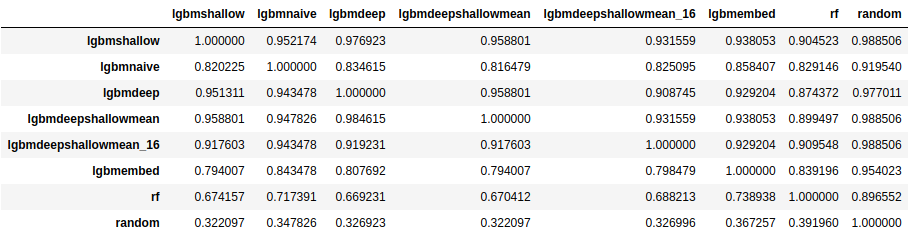
\includegraphics[width=\linewidth]{model_dependencies.png}
  \caption{
    $a_{i,j} = \frac{|T_i \cap T_j|}{|T_j|}$,
$ T_i $ - Set of theorems proved by model $i$
  }
  \label{fig:modelsims}
\end{figure}
.\newline
Figure 1 shows how many (\%) of j theorems (proved by model j) are proved by model i. $a_{i,j} = 1$ means that model i is at every aspect better (not worse) then model j (proved all his theorems).There is no nontrivial occurences of that.

As you can see even random permutation of premises isn't totally covered by any of the models and none of them is actually even really close. This suggests a lot of space for improvements.

\section{Next Steps}
\begin{itemize}
\item \textbf{More models tested} - For example simple Regression (maybe on embeddings with polynomial features) could model different thing and help increasing at least sum of all theorems proved. 
\item \textbf{Training only on short proofs} - One can think that if there are many premises are in the proof, then they aren't that relevant and probably many of them are useful only with a combination of an other premise. Therefore we can just use short proofs for training that probably use simple relationships for inferences - the type we're looking for.
\item \textbf{Regression} - This is an extension of the previous one. instead of classification we can train a regressor that in a simplest case scenario just sums up all the occurences of the premise for a given theorem, but one could also weight the premises by the inverse of the number of premises used for a proof, so if proof uses 3 premises to proof theorem then their weights are equal to 1/3. And for a pair (theorem,premise) we sum all the weights and train regression on that.
\item \textbf{Iterative training} - theorems that are proved can later be used as samples for new training sets, which gets bigger with every iteration.
\item \textbf{Hyperparameters} - There are a lot of parameters in the training. From lgbm parameters to 'meta-parameters': \begin{itemize}
	\item Ratio of False to True samples in training dataset - setting it higher would probably improve results, as it would better resolve real scenario.
	\item number of trees
	\item trees depth
	\item regularization
	\end{itemize}
\item \textbf{Embeddings with theorem-premises list} - Instead of creating embeddings with features one could try creating them with list of theorems and their respective premises.
\item \textbf{More stubborn prediction with dynamic number of premises} - For now the program doesn't even check whether solver gave up (timeout) or didn't manage to solve (not enough premises). It could check it and increase number (start with small numbers) of premises until it finds proof or times out. That's important because for some theorems it may be sufficient to choose 2 premises, but for some many premises are needed. It's impossible to model with current architecture.
\item \textbf{Ignored Set Dependencies} - for now we look only at pairs (Theorem, Premise), but it might be the case that 2 (or more) premises are useful for some theorem only when they're together.
\item \textbf{Better Features} - Using semantic dependencies between features or at least extracting more semantic features (as with autoencoder attempt).
\item \textbf{Recommender System approach} - This setup is very similar to the recommender system approach. We are literally recommending a SAT solver set of premises. I'd like to try some RecSyss approaches which could for example help with the problem of ignored set dependencies (even basic like apriori algorithms, although that definitely be too simple).

\end{itemize}

\section{Conclusion}

Despite using only syntactic features which are obfuscated and many shortcuts taken along the way models seem to be quite useful in helping selecting the best premises. There is still a huge space for improvement which is shown in previous chapter. I estimate that with these improvements model could reach 85\% - 90\% of theorems coverage.

\end{document}